\section{Introduction}
\label{sec:introduction}

Large language models have emerged as powerful components in evolutionary search, replacing hand-crafted mutation operators~\citep{o2010open} with learned code generation~\citep{lehman2022elm, funsearch2024, alphaevolve2025, chen2023evoprompting}.
In these systems, an LLM generates candidate solutions conditioned on selected parents, while a surrounding framework, which is usually heuristic-based, handles parent sampling, evaluation, and population management.
This combination has produced notable results in mathematical optimization and algorithm discovery, including flagship systems such as FunSearch and AlphaEvolve~\citep{funsearch2024, alphaevolve2025}.
However, confining the LLM to candidate generation within a prescribed pipeline fundamentally limits what the LLM can discover: it produces a single output per invocation, with no ability to proactively consult reference materials, test its changes, interpret feedback, or revise its approach before committing a candidate.
For the most aggressively hand-tuned implementations, where further improvement requires deep, iterative engineering, this constraint is especially limiting.

We study this problem in the context of attention~\citep{vaswani2017attention}, the central operation in Transformer architectures, and one of the most heavily optimized GPU kernels.
The FlashAttention lineage~\citep{dao2022flashattention, dao2024flashattention2, shah2024flashattention3, zadouri2026flashattention4} and NVIDIA's cuDNN library~\citep{chetlur2014cudnn} have pushed attention throughput progressively closer to hardware limits across successive GPU generations, with both FlashAttention-4 (FA4) and cuDNN requiring months of manual optimization on the latest Blackwell architecture.
Surpassing these implementations demands sustained, iterative interaction with the development environment: studying hardware documentation, analyzing profiler output to identify bottlenecks, implementing and testing candidate optimizations, diagnosing correctness failures, and revising strategy based on accumulated experience.

\begin{figure}[t]
  \centering
    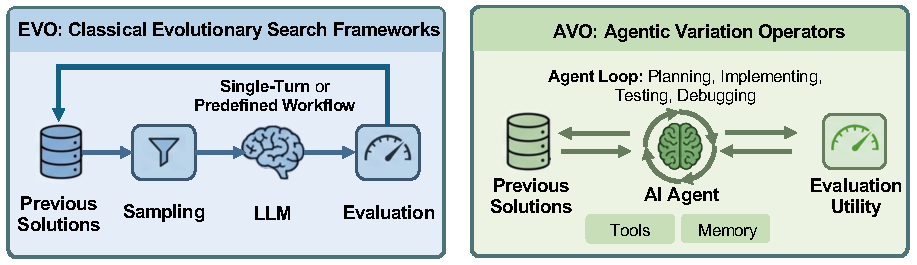
\includegraphics[width=0.9\textwidth]{figures/teaser.pdf}
  \caption{\textbf{EVO vs AVO}: Comparison between prior evolutionary search frameworks (e.g. FunSearch, AlphaEvolve, and related LLM-augmented evolutionary approaches) and the proposed Agentic Variation Operator. \textbf{Left:} Prior approaches follow a fixed pipeline where the LLM is confined to a single-turn generation step or a predefined workflow, with sampling and evaluation controlled by the framework. \textbf{Right:} AVO replaces this pipeline with an autonomous AI agent that iteratively plans, implements, tests, and debugs across long-running sessions, with direct access to previous solutions, evaluation utilities, tools, and persistent memory.}
  \label{fig:teaser}
\end{figure}

Recent progress in \emph{deep agents}~\citep{jimenez2024swebench, yang2024sweagent, wang2024openhands, anthropic2025cc, openai2025codex} demonstrates that LLMs augmented with planning, persistent memory, and tool use can autonomously navigate such multi-step engineering workflows, with applications ranging from resolving complex GitHub issues to generating key deep learning software~\citep{xu2026vibetensor}.
This motivates a fundamentally different role for LLMs in evolutionary search: rather than confining them within a fixed pipeline, we can elevate a deep agent to serve as the variation operator itself.
To this end, we propose \textbf{Agentic Variation Operators (AVO)}, in which a self-directed coding agent replaces the mutation and crossover process in previous works based on single-turn LLMs~\citep{funsearch2024, alphaevolve2025, chen2023evoprompting} or fixed workflows~\citep{wan2025loongflow}.
The AVO agent has access to all prior solutions, a domain-specific knowledge base, and the evaluation utility.
It autonomously decides what to consult, what to edit, and when to evaluate, enabling continuous improvements over extended time horizons.

To demonstrate its effectiveness, we apply AVO to multi-head attention (MHA) kernels on the Blackwell B200 GPU, and directly compare against the expert-optimized cuDNN and FlashAttention-4 kernels.
Over 7 days of continuous evolution without human intervention, the agent explored over 500 optimization directions and evolved 40 kernel versions, producing MHA kernels achieving up to 1668 TFLOPS at BF16 precision, outperforming cuDNN by up to 3.5\% and FlashAttention-4 by up to 10.5\%.
Our analysis of agent-discovered optimizations reveals that they span multiple levels of kernel design, including register allocation, instruction pipeline scheduling, and workload distribution, reflecting genuine hardware-level reasoning.
Empirically, we find that the optimization techniques discovered on MHA transfer effectively to grouped-query attention (GQA): adapting the evolved MHA kernel to support GQA requires only 30 minutes of additional autonomous agent effort, yielding up to 7.0\% performance improvement over cuDNN and 9.3\% over FlashAttention-4.



Our contributions are as follows:
\begin{itemize}
    \item We introduce Agentic Variation Operators (AVO), a new family of evolutionary variation operators that elevate the agent from candidate generator to variation operator, autonomously exploring domain knowledge, implementing edits, and validating results through iterative interaction with the environment.
    \item We achieve state-of-the-art MHA throughput on NVIDIA B200 GPUs across the benchmarked configurations, reaching up to 1668 TFLOPS and outperforming cuDNN by up to 3.5\% and FlashAttention-4 by up to 10.5\%. Furthermore, we show that the discovered optimizations readily transfer to GQA, requiring only 30 minutes of autonomous adaptation and yielding gains of up to 7.0\% over cuDNN and 9.3\% over FlashAttention-4.
    \item We provide a detailed analysis of the micro-architectural optimizations discovered by the agent under the benchmarked settings, showing the agent performs genuine hardware-level reasoning rather than superficial code transformations.
\end{itemize}
